\documentclass{article}

% content/resources/templates/preamble.tex
\usepackage[margin=0.6in]{geometry}
\author{Milav Dabgar}
\usepackage{amsmath,amssymb,amsthm}
\usepackage{booktabs}
\usepackage{multirow}
\usepackage{xcolor}
\usepackage{tcolorbox}
\tcbuselibrary{breakable,skins}
\usepackage[colorlinks=true,linkcolor=blue]{hyperref}
\usepackage{titlesec}
\usepackage{enumitem}
\usepackage{tikz}
\usepackage{pgfplots}
\usepackage{circuitikz}
\usepackage[version=4]{mhchem}
\usepackage{longtable}
\usepackage{array}
\usepackage{float}
\usepackage{caption}
\usepackage{listings}

\lstset{
  basicstyle=\small\ttfamily,
  breaklines=true,
  breakatwhitespace=false,
  postbreak=\mbox{\textcolor{red}{$\hookrightarrow$}\space},
  float=false,
  numbers=left,
  numberstyle=\tiny\color{gray},
  numbersep=10pt,
  xleftmargin=2em,
  keywordstyle=\color{blue},
  commentstyle=\color{green!60!black},
  stringstyle=\color{purple},
  backgroundcolor=\color{gray!5},
  showstringspaces=false,
  tabsize=2,
  captionpos=b,
  keepspaces=true,
  columns=flexible
}

\pgfplotsset{compat=1.18}
\usetikzlibrary{shapes,arrows,positioning,calc,patterns,decorations.pathmorphing,decorations.markings,arrows.meta}

% Color scheme
\definecolor{headcolor}{RGB}{0,102,204}
\definecolor{keycolor}{RGB}{220,20,60}
\definecolor{solutioncolor}{RGB}{34,139,34}
\definecolor{mnemoniccolor}{RGB}{148,0,211}
\definecolor{codecolor}{RGB}{0,0,100}

% Spacing
\setlength{\parskip}{3pt}
\setlist[itemize]{nosep}
\setlist[enumerate]{nosep}

% Title formatting
\titleformat{\section}{\Large\bfseries\color{headcolor}}{\thesection}{1em}{}
\titleformat{\subsection}{\large\bfseries\color{headcolor}}{\thesubsection}{1em}{}

% Pandoc tightlist compatibility
\providecommand{\tightlist}{%
  \setlength{\itemsep}{0pt}\setlength{\parskip}{0pt}}

% Pandoc longtable compatibility
\newcounter{none}
\def\thenone{}


% content/resources/templates/english-boxes.tex

% Custom environments
\newtcolorbox{solutionbox}{
 breakable,
 enhanced,
 colback=solutioncolor!5!white,
 colframe=solutioncolor!75!black,
 fonttitle=\bfseries,
 title=Solution
}

\newtcolorbox{solutionboxnobreak}{
 colback=solutioncolor!5!white,
 colframe=solutioncolor!75!black,
 fonttitle=\bfseries,
 title=Solution
}

\newtcolorbox{keyformula}{
 breakable,
 enhanced,
 colback=keycolor!5!white,
 colframe=keycolor!75!black,
 fonttitle=\bfseries,
 title=Key Formula
}

\newtcolorbox{mnemonicboxenv}{
 breakable,
 enhanced,
 colback=mnemoniccolor!5!white,
 colframe=mnemoniccolor!75!black,
 fonttitle=\bfseries,
 title=Mnemonic
}

\newcommand{\mnemonicbox}[1]{%
  \begin{mnemonicboxenv}
    #1
  \end{mnemonicboxenv}
}


% Custom commands for GTU solutions
% This file defines semantic commands for consistent formatting

% Question command with automatic formatting
\newcommand{\question}[2]{%
  \section*{Question #1}%
  \textbf{#2}%
}

% OR question variant
\newcommand{\questionor}[2]{%
  \section*{Question #1 OR}%
  \textbf{#2}%
}

% Proper table environment with caption
\newenvironment{answertable}[1]{%
  \begin{table}[htbp]
  \centering
  \caption{#1}
}{%
  \end{table}
}

% Proper figure environment for diagrams
\newenvironment{answerdiagram}[1]{%
  \begin{figure}[htbp]
  \centering
  \caption{#1}
}{%
  \end{figure}
}

% Semantic markup for key terms
\newcommand{\keyword}[1]{\textbf{#1}}
\newcommand{\code}[1]{\texttt{#1}}
\newcommand{\classname}[1]{\texttt{#1}}
\newcommand{\methodname}[1]{\texttt{#1}}

% Proper quotation marks
\newcommand{\mnemonic}[1]{``#1''}


\title{Communication Engineering (1333201) - Summer 2024 Solution}
\date{June 06, 2024}

\begin{document}
\maketitle

\questionmarks{1(a)}{3}{Define modulation and explain its need.}

\begin{solutionbox}
\textbf{Answer}:
Modulation is the process of varying one or more properties of a high-frequency carrier signal with a modulating signal containing information.

\begin{center}
\captionof{table}{Need for Modulation}
\begin{tabulary}{\linewidth}{|L|L|}
\hline
\textbf{Need} & \textbf{Explanation} \\
\hline
\textbf{Antenna Size Reduction} & Allows practical antenna size ($\lambda/4$) by increasing frequency \\
\hline
\textbf{Signal Propagation} & Higher frequencies travel farther through atmosphere \\
\hline
\textbf{Multiplexing} & Allows multiple signals to be transmitted simultaneously \\
\hline
\textbf{Interference Reduction} & Shifts signal to band with less noise/interference \\
\hline
\textbf{Bandwidth Allocation} & Enables efficient spectrum usage by different services \\
\hline
\end{tabulary}
\end{center}
\end{solutionbox}

\begin{mnemonicbox}
"ASPIM" - Antenna size, Signal propagation, Proper multiplexing, Interference reduction, Manage bandwidth
\end{mnemonicbox}

\questionmarks{1(b)}{4}{Draw \& explain block diagram of Communication system}

\begin{solutionbox}
\textbf{Answer}:
A communication system transfers information from source to destination through a channel.

\begin{center}
\begin{tikzpicture}[node distance=2.5cm, auto, >=latex, thick]
    % Nodes
    \node [gtu block] (source) {Information\\Source};
    \node [gtu block, right of=source] (tx) {Transmitter};
    \node [gtu block, right of=tx] (channel) {Channel};
    \node [gtu block, right of=channel] (rx) {Receiver};
    \node [gtu block, right of=rx] (dest) {Destination};
    \node [gtu block, below of=channel, node distance=2cm] (noise) {Noise Source};

    % Arrows
    \draw [gtu arrow] (source) -- (tx);
    \draw [gtu arrow] (tx) -- (channel);
    \draw [gtu arrow] (channel) -- (rx);
    \draw [gtu arrow] (rx) -- (dest);
    \draw [gtu arrow] (noise) -- (channel);
\end{tikzpicture}
\captionof{figure}{Communication System Block Diagram}
\end{center}

\begin{center}
\captionof{table}{Communication System Components}
\begin{tabulary}{\linewidth}{|L|L|}
\hline
\textbf{Component} & \textbf{Function} \\
\hline
\textbf{Information Source} & Produces message to be transmitted (voice, video, data) \\
\hline
\textbf{Transmitter} & Converts message to suitable signals (modulation, coding) \\
\hline
\textbf{Channel} & Medium through which signals travel (wire, fiber, air) \\
\hline
\textbf{Noise Source} & Unwanted signals that corrupt the transmitted signal \\
\hline
\textbf{Receiver} & Extracts original message from received signal (demodulation) \\
\hline
\textbf{Destination} & Where the message is delivered (human, machine) \\
\hline
\end{tabulary}
\end{center}
\end{solutionbox}

\begin{mnemonicbox}
"I Try Communicating Neatly, Receive Data" (I-T-C-N-R-D)
\end{mnemonicbox}

\questionmarks{1(c)}{7}{Derive voltage equation for Amplitude modulation.}

\begin{solutionbox}
\textbf{Answer}:
Amplitude modulation varies the amplitude of carrier signal proportionally to the message signal.

\textbf{Mathematical Derivation:}
\begin{itemize}
    \item Let carrier signal be: $c(t) = A_c \cos(\omega_c t)$
    \item Message signal: $m(t) = A_m \cos(\omega_m t)$
    \item AM signal: $s(t) = A_c[1 + \mu \cdot m(t)/A_m]\cos(\omega_c t)$
    \item Where $\mu = \text{modulation index} = A_m/A_c$
    \item Substituting $m(t)$: $s(t) = A_c[1 + \mu \cdot \cos(\omega_m t)]\cos(\omega_c t)$
    \item Expanding: $s(t) = A_c \cdot \cos(\omega_c t) + \mu \cdot A_c \cdot \cos(\omega_m t) \cdot \cos(\omega_c t)$
    \item Using identity ($\cos A \cdot \cos B$): $s(t) = A_c \cdot \cos(\omega_c t) + (\frac{\mu A_c}{2})[\cos(\omega_c + \omega_m)t + \cos(\omega_c - \omega_m)t]$
\end{itemize}

\begin{center}
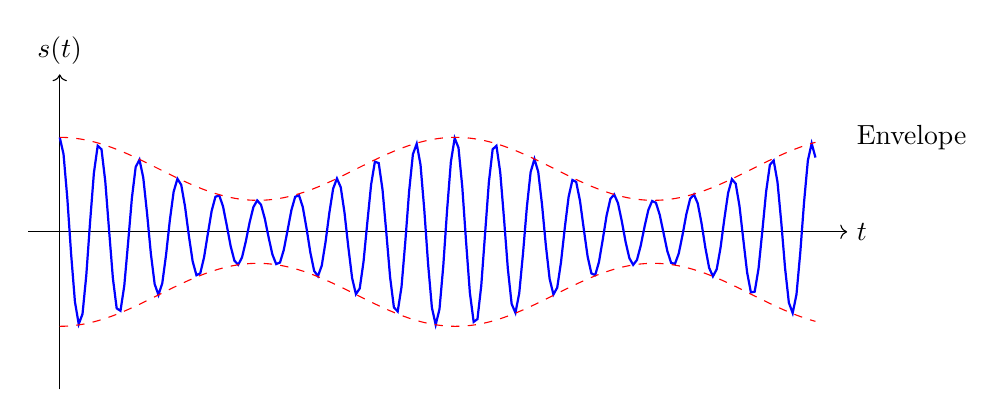
\begin{tikzpicture}[domain=0:12, samples=200, scale=0.8]
    \draw[->] (-0.5,0) -- (12.5,0) node[right] {$t$};
    \draw[->] (0,-2.5) -- (0,2.5) node[above] {$s(t)$};
    
    % AM Signal: (1 + 0.5cos(t)) * cos(10t)
    \draw[blue, thick] plot (\x, {(1 + 0.5*cos(\x r)) * cos(10*\x r)});
    \draw[red, dashed] plot (\x, {1 + 0.5*cos(\x r)});
    \draw[red, dashed] plot (\x, {-1 - 0.5*cos(\x r)});
    
    \node[right] at (12.5, 1.5) {Envelope};
\end{tikzpicture}
\captionof{figure}{AM Signal in Time Domain}
\end{center}
\end{solutionbox}

\begin{mnemonicbox}
"CAMDS" - Carrier Amplitude Modulated by Data Signal
\end{mnemonicbox}

\questionmarks{1(c) OR}{7}{Derive the equation for total power in AM, calculate percentage of power savings in DSB and SSB.}

\begin{solutionbox}
\textbf{Answer}:
For an AM signal with modulation index $\mu$, the total power consists of carrier power and sideband power.

\begin{center}
\captionof{table}{Power Distribution in AM}
\begin{tabulary}{\linewidth}{|L|L|L|}
\hline
\textbf{Component} & \textbf{Power Formula} & \textbf{Percentage of Total Power} \\
\hline
Carrier & $P_c = A_c^2/2$ & $1/(1+\mu^2/2) \times 100\%$ \\
\hline
Upper Sideband & $P_{USB} = P_c \cdot \mu^2/4$ & $(\mu^2/4)/(1+\mu^2/2) \times 100\%$ \\
\hline
Lower Sideband & $P_{LSB} = P_c \cdot \mu^2/4$ & $(\mu^2/4)/(1+\mu^2/2) \times 100\%$ \\
\hline
Total & $P_T = P_c(1+\mu^2/2)$ & $100\%$ \\
\hline
\end{tabulary}
\end{center}

\textbf{Power Savings Calculation:}
\begin{itemize}
    \item In DSB-SC: 100\% carrier suppression = $(P_c/P_T) \times 100\% = 1/(1+\mu^2/2) \times 100\%$
    \begin{itemize}
        \item For $\mu = 1$: Saving = $2/3 \times 100\% = 66.67\%$
    \end{itemize}
    \item In SSB: One sideband + carrier suppression = $(P_c+P_{LSB})/P_T \times 100\% = (1+\mu^2/4)/(1+\mu^2/2) \times 100\%$
    \begin{itemize}
        \item For $\mu = 1$: Saving = $5/6 \times 100\% = 83.33\%$
    \end{itemize}
\end{itemize}
\end{solutionbox}

\begin{mnemonicbox}
"CAPS" - Carrier And Power in Sidebands
\end{mnemonicbox}

\questionmarks{2(a)}{3}{Define Image frequency in a radio receiver and explain it with suitable example.}

\begin{solutionbox}
\textbf{Answer}:
Image frequency is an unwanted frequency that can produce the same IF (Intermediate Frequency) as the desired signal in a superheterodyne receiver.

\begin{center}
\begin{table}[H]
\centering
\begin{tabulary}{\textwidth}{|L|L|L|}
\hline
\textbf{Parameter} & \textbf{Formula} & \textbf{Example} \\
\hline
\textbf{Desired Signal} & $f_s$ & 100 MHz \\
\hline
\textbf{Local Oscillator} & $f_{LO}$ & 110 MHz \\
\hline
\textbf{IF} & $f_{IF} = f_{LO} - f_s$ & 10 MHz \\
\hline
\textbf{Image Frequency} & $f_{image} = f_{LO} + f_{IF}$ & 120 MHz \\
\hline
\end{tabulary}
\caption{Image Frequency}
\end{table}
\end{center}

If both 100 MHz and 120 MHz signals exist, both will produce 10 MHz IF, causing interference.
\end{solutionbox}

\begin{mnemonicbox}
"LIDS" - Local oscillator plus/minus IF gives Desired signal and Signal image
\end{mnemonicbox}

\questionmarks{2(b)}{4}{Draw and explain block diagram for envelope detector.}

\begin{solutionbox}
\textbf{Answer}:
Envelope detector extracts the modulating signal from AM wave by following the envelope.

\begin{center}
\begin{figure}[H]
\centering
\begin{tikzpicture}[auto, >=latex, thick]
    \node (input) {AM Input};
    \node [right of=input, node distance=2cm] (diode) {};
    % Diode symbol
    \draw (diode) -- ++(1,0) coordinate (d1);
    \draw (d1) -- ++(0.5,0.5) -- ++(0,-1) -- ++(-0.5,0.5); 
    \draw (d1) ++(0.5,-0.5) -- ++(0,1);
    \draw (d1) ++(0.5,0) -- ++(1,0) coordinate (node1);
    
    % RC parallel
    \draw (node1) -- ++(0,-1.5) coordinate (c_top);
    \draw (c_top) to[C, l=C] ++(0,-1.5) coordinate (gnd);
    \draw (node1) -- ++(2,0) coordinate (node2);
    \draw (node2) -- ++(0,-1.5) coordinate (r_top);
    \draw (r_top) to[R, l=R] ++(0,-1.5) coordinate (gnd2);
    
    % Ground
    \node [ground] at (gnd) {};
    \node [ground] at (gnd2) {};
    
    % Output
    \draw (node2) -- ++(1.5,0) node[right] (output) {Envelope Output};
    
    \node [above of=diode] {Diode};
\end{tikzpicture}
\captionof{figure}{Envelope Detector}
\end{figure}
\end{center}

\begin{center}
\captionof{table}{Envelope Detector Components}
\begin{tabulary}{\textwidth}{|L|L|}
\hline
\textbf{Component} & \textbf{Function} \\
\hline
\textbf{Diode} & Rectifies the AM signal (passes positive half) \\
\hline
\textbf{Capacitor} & Charges to peak value of rectified signal \\
\hline
\textbf{Resistor} & Discharges capacitor with time constant RC \\
\hline
\textbf{RC Value} & $1/\omega_m < RC < 1/\omega_c$ (where $\omega_m$ is message frequency, $\omega_c$ is carrier) \\
\hline
\end{tabulary}
\end{center}
\end{solutionbox}

\begin{mnemonicbox}
"DRCT" - Diode Rectifies, Capacitor Tracks
\end{mnemonicbox}

\questionmarks{2(c)}{7}{Draw block diagram of AM radio receiver and explain working of each block.}

\begin{solutionbox}
\textbf{Answer}:
AM receiver converts radio signal to audio output.

\begin{center}
\begin{tikzpicture}[node distance=2cm, auto, >=latex, thick, scale=0.8, transform shape]
    \node [gtu block] (ant) {Antenna};
    \node [gtu block, right of=ant, node distance=2.5cm] (rf) {RF Amp};
    \node [gtu block, right of=rf, node distance=2.5cm] (mix) {Mixer};
    \node [gtu block, below of=mix] (lo) {Local Osc};
    \node [gtu block, right of=mix, node distance=2.5cm] (if) {IF Amp};
    \node [gtu block, right of=if, node distance=2.5cm] (det) {Detector};
    \node [gtu block, right of=det, node distance=2.5cm] (af) {AF Amp};
    \node [gtu block, right of=af, node distance=2.5cm] (spk) {Speaker};

    \draw [gtu arrow] (ant) -- (rf);
    \draw [gtu arrow] (rf) -- (mix);
    \draw [gtu arrow] (lo) -- (mix);
    \draw [gtu arrow] (mix) -- (if);
    \draw [gtu arrow] (if) -- (det);
    \draw [gtu arrow] (det) -- (af);
    \draw [gtu arrow] (af) -- (spk);
\end{tikzpicture}
\captionof{figure}{AM Receiver Block Diagram}
\end{center}

\begin{center}
\captionof{table}{AM Receiver Blocks}
\begin{tabulary}{\textwidth}{|L|L|}
\hline
\textbf{Block} & \textbf{Function} \\
\hline
\textbf{Antenna} & Captures electromagnetic signals from air \\
\hline
\textbf{RF Amplifier} & Amplifies weak RF signals, provides selectivity \\
\hline
\textbf{Local Oscillator} & Generates frequency to mix with incoming signal \\
\hline
\textbf{Mixer} & Combines RF and oscillator signals to produce IF \\
\hline
\textbf{IF Amplifier} & Amplifies fixed IF signal with high gain \\
\hline
\textbf{Detector} & Extracts audio signal from AM carrier \\
\hline
\textbf{AF Amplifier} & Boosts audio signal power to drive speaker \\
\hline
\textbf{Speaker} & Converts electrical signal to sound \\
\hline
\end{tabulary}
\end{center}
\end{solutionbox}

\begin{mnemonicbox}
"ARMLIDAS" - Antenna Receives, Mixer Links Input and Detector, Audio to Speaker
\end{mnemonicbox}

\questionmarks{2(a) OR}{3}{Define any FOUR characteristics of radio receiver.}

\begin{solutionbox}
\textbf{Answer}:
\begin{center}
\captionof{table}{Radio Receiver Characteristics}
\begin{tabulary}{\linewidth}{|L|L|}
\hline
\textbf{Characteristic} & \textbf{Definition} \\
\hline
\textbf{Sensitivity} & Minimum signal strength that produces standard output \\
\hline
\textbf{Selectivity} & Ability to separate desired signal from adjacent channels \\
\hline
\textbf{Fidelity} & Accuracy of reproducing original modulating signal \\
\hline
\textbf{Image Rejection} & Ability to reject image frequency signals \\
\hline
\textbf{Signal-to-Noise Ratio} & Ratio of desired signal power to noise power \\
\hline
\end{tabulary}
\end{center}
\end{solutionbox}

\begin{mnemonicbox}
"SSFIS" - Super Sensitive Fidelity with Image Suppression
\end{mnemonicbox}

\questionmarks{2(b) OR}{4}{Explain Ratio detector circuit for FM detection.}

\begin{solutionbox}
\textbf{Answer}:
Ratio detector extracts audio from FM signals while rejecting amplitude variations.

\begin{center}
\begin{tikzpicture}[auto, >=latex, thick]
    % Simplified representation
    \node [gtu block] (input) {FM Input / Transformer};
    \node [gtu block, right of=input, node distance=3.5cm] (diodes) {Diode Bridge (Opposite)};
    \node [gtu block, right of=diodes, node distance=3.5cm] (cap) {Large Cap ($10\mu F$)};
    \node [gtu block, right of=cap, node distance=3.5cm] (out) {Audio Output};

    \draw [gtu arrow] (input) -- (diodes);
    \draw [gtu arrow] (diodes) -- (cap);
    \draw [gtu arrow] (cap) -- (out);
\end{tikzpicture}
\captionof{figure}{Ratio Detector Block Diagram}
\end{center}

\begin{center}
\captionof{table}{Ratio Detector Components}
\begin{tabulary}{\linewidth}{|L|L|}
\hline
\textbf{Component} & \textbf{Function} \\
\hline
\textbf{Transformer} & Creates phase shifts proportional to frequency deviation \\
\hline
\textbf{Diodes} & Arranged in opposite polarity to produce voltage ratio \\
\hline
\textbf{Stabilizing Capacitor} & Large value ($10\mu F$) to suppress AM variations \\
\hline
\textbf{RC Network} & Extracts the audio signal from ratio of voltages \\
\hline
\end{tabulary}
\end{center}
\end{solutionbox}

\begin{mnemonicbox}
"RADS" - Ratio detector Avoids Disturbance from Strength variations
\end{mnemonicbox}

\questionmarks{2(c) OR}{7}{Draw and explain block diagram of super heterodyne receiver.}

\begin{solutionbox}
\textbf{Answer}:
Superheterodyne receiver converts all incoming RF to fixed IF for better amplification.

\begin{center}
\begin{tikzpicture}[node distance=2cm, auto, >=latex, thick, scale=0.8, transform shape]
    \node [gtu block] (ant) {Antenna};
    \node [gtu block, right of=ant, node distance=2.2cm] (rf) {RF Amp};
    \node [gtu block, right of=rf, node distance=2.2cm] (mix) {Mixer};
    \node [gtu block, below of=mix] (lo) {Local Osc};
    \node [gtu block, right of=mix, node distance=2.2cm] (if) {IF Amp};
    \node [gtu block, right of=if, node distance=2.2cm] (det) {Detector};
    \node [gtu block, below of=det] (agc) {AGC};
    \node [gtu block, right of=det, node distance=2.2cm] (af) {AF Amp};
    \node [gtu block, right of=af, node distance=2.2cm] (spk) {Speaker};

    \draw [gtu arrow] (ant) -- (rf);
    \draw [gtu arrow] (rf) -- (mix);
    \draw [gtu arrow] (lo) -- (mix);
    \draw [gtu arrow] (mix) -- (if);
    \draw [gtu arrow] (if) -- (det);
    \draw [gtu arrow] (det) -- (af);
    \draw [gtu arrow] (af) -- (spk);
    
    % AGC feedback
    \draw [gtu arrow] (det) -- (agc);
    \draw [gtu arrow] (agc) -| (if);
    \draw [gtu arrow] (agc) -| (rf);
\end{tikzpicture}
\captionof{figure}{Superheterodyne Receiver Block Diagram}
\end{center}

\begin{center}
\captionof{table}{Superheterodyne Receiver Components}
\begin{tabulary}{\linewidth}{|L|L|}
\hline
\textbf{Block} & \textbf{Function} \\
\hline
\textbf{Antenna} & Captures RF signals \\
\hline
\textbf{RF Amplifier} & Amplifies and selects desired frequency band \\
\hline
\textbf{Local Oscillator} & Generates frequency above/below signal by IF value \\
\hline
\textbf{Mixer} & Heterodynes signal and oscillator to produce IF \\
\hline
\textbf{IF Amplifier} & Provides most gain and selectivity at fixed frequency \\
\hline
\textbf{Detector} & Recovers original modulating signal \\
\hline
\textbf{AGC} & Automatic Gain Control - maintains constant output level \\
\hline
\textbf{AF Amplifier} & Amplifies audio to drive speaker \\
\hline
\textbf{Speaker} & Converts electrical signal to sound \\
\hline
\end{tabulary}
\end{center}
\end{solutionbox}

\begin{mnemonicbox}
"ARMLIADS" - Antenna Receives, Mixer Links, Intermediate Amplifies, Detector Separates
\end{mnemonicbox}

\questionmarks{3(a)}{3}{Draw the Time and frequency domain representation of the below signals. 1. Analog signal (sine) 2. Digital signal (square).}

\begin{solutionbox}
\textbf{Answer}:

\begin{center}
\begin{tabulary}{\textwidth}{|L|L|L|}
\hline
\textbf{Signal Type} & \textbf{Time Domain} & \textbf{Frequency Domain} \\
\hline
\textbf{Sine Wave} & Sinusoidal curve & Single spike at frequency f \\
\hline
\textbf{Square Wave} & Alternating levels & Fundamental and odd harmonics ($1/n$ pattern) \\
\hline
\end{tabulary}
\captionof{table}{Signal Representations}
\end{center}

\begin{center}
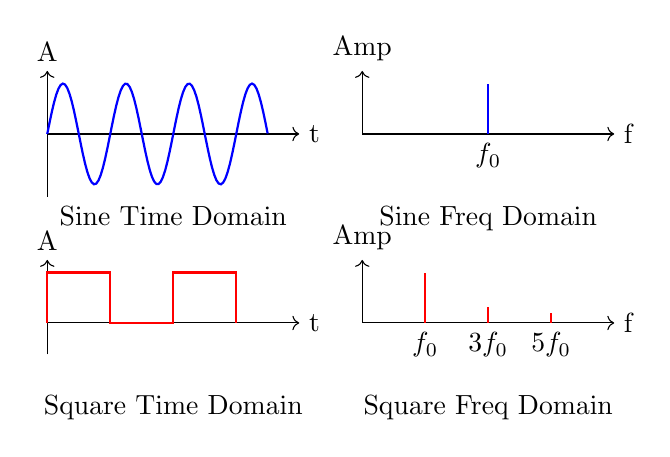
\begin{tikzpicture}[scale=0.8]
    % Sine Time
    \begin{scope}[xshift=0cm, yshift=3cm]
        \draw[->] (0,0) -- (4,0) node[right] {t};
        \draw[->] (0,-1) -- (0,1) node[above] {A};
        \draw[blue, thick, domain=0:3.5, samples=100] plot (\x, {0.8*sin(360*\x)});
        \node[below] at (2,-1) {Sine Time Domain};
    \end{scope}

    % Sine Freq
    \begin{scope}[xshift=5cm, yshift=3cm]
        \draw[->] (0,0) -- (4,0) node[right] {f};
        \draw[->] (0,0) -- (0,1) node[above] {Amp};
        \draw[blue, thick] (2,0) -- (2,0.8);
        \node[below] at (2,0) {$f_0$};
        \node[below] at (2,-1) {Sine Freq Domain};
    \end{scope}

    % Square Time
    \begin{scope}[xshift=0cm, yshift=0cm]
        \draw[->] (0,0) -- (4,0) node[right] {t};
        \draw[->] (0,-0.5) -- (0,1) node[above] {A};
        \draw[red, thick] (0,0) -- (0,0.8) -- (1,0.8) -- (1,0) -- (2,0) -- (2,0.8) -- (3,0.8) -- (3,0);
        \node[below] at (2,-1) {Square Time Domain};
    \end{scope}

    % Square Freq
    \begin{scope}[xshift=5cm, yshift=0cm]
        \draw[->] (0,0) -- (4,0) node[right] {f};
        \draw[->] (0,0) -- (0,1) node[above] {Amp};
        \draw[red, thick] (1,0) -- (1,0.8);
        \draw[red, thick] (2,0) -- (2,0.26); % 1/3
        \draw[red, thick] (3,0) -- (3,0.16); % 1/5
        \node[below] at (1,0) {$f_0$};
        \node[below] at (2,0) {$3f_0$};
        \node[below] at (3,0) {$5f_0$};
        \node[below] at (2,-1) {Square Freq Domain};
    \end{scope}
\end{tikzpicture}
\captionof{figure}{Signal Representations}
\end{center}
\end{solutionbox}

\begin{mnemonicbox}
"SOFT" - Sine has One Frequency, square has Timeless harmonics
\end{mnemonicbox}

\questionmarks{3(b)}{4}{Explain sampling theorem.}

\begin{solutionbox}
\textbf{Answer}:
Sampling theorem states the conditions for accurate signal reconstruction from samples.

\begin{center}
\begin{tabulary}{\textwidth}{|L|L|}
\hline
\textbf{Aspect} & \textbf{Description} \\
\hline
\textbf{Statement} & To reconstruct a signal perfectly, sampling frequency must be at least twice the highest frequency in signal \\
\hline
\textbf{Nyquist Rate} & $f_s \ge 2f_{max}$ (minimum sampling frequency) \\
\hline
\textbf{Aliasing} & Distortion that occurs when sampling below Nyquist rate \\
\hline
\textbf{Example} & For voice (300-3400 Hz), $f_s \ge 6.8$ kHz (typically 8 kHz) \\
\hline
\end{tabulary}
\captionof{table}{Sampling Theorem}
\end{center}

\begin{center}
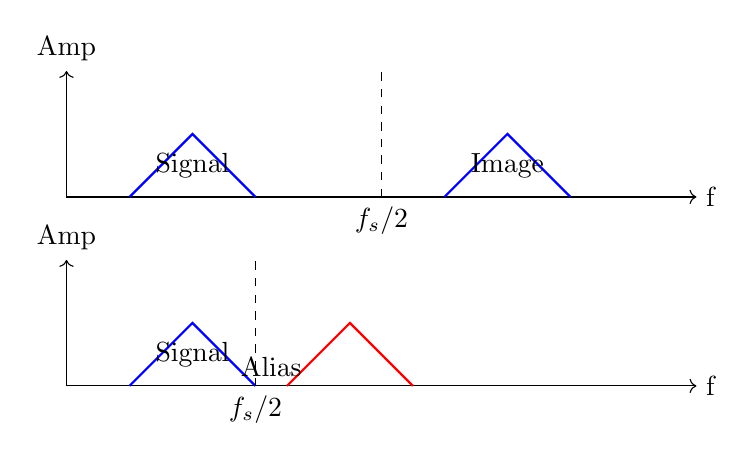
\begin{tikzpicture}[scale=0.8]
    \draw[->] (0,0) -- (10,0) node[right] {f};
    \draw[->] (0,0) -- (0,2) node[above] {Amp};
    
    % Proper Sampling
    \draw[blue, thick] (1,0) -- (2,1) -- (3,0);
    \node at (2,0.5) {Signal};
    \draw[blue, thick] (6,0) -- (7,1) -- (8,0);
    \node at (7,0.5) {Image};
    \node[below] at (5,0) {$f_s/2$};
    \draw[dashed] (5,0) -- (5,2);
    
    % Aliasing
    \begin{scope}[yshift=-3cm]
        \draw[->] (0,0) -- (10,0) node[right] {f};
        \draw[->] (0,0) -- (0,2) node[above] {Amp};
        \draw[blue, thick] (1,0) -- (2,1) -- (3,0);
        \draw[red, thick] (3.5,0) -- (4.5,1) -- (5.5,0); % Shifted left causing overlap
        \node at (2,0.5) {Signal};
        \node at (3.25, 0.3) {Alias};
        \node[below] at (3,0) {$f_s/2$};
        \draw[dashed] (3,0) -- (3,2);
    \end{scope}
\end{tikzpicture}
\captionof{figure}{Aliasing Effect}
\end{center}
\end{solutionbox}

\begin{mnemonicbox}
"SNAP" - Sample at Nyquist And Prevent aliasing
\end{mnemonicbox}

\questionmarks{3(c)}{7}{Explain PAM, PPM and PWM.}

\begin{solutionbox}
\textbf{Answer}:
These are pulse modulation techniques where a parameter of pulse is varied.

\begin{center}
\begin{tabulary}{\textwidth}{|L|L|L|L|}
\hline
\textbf{Type} & \textbf{Full Form} & \textbf{Parameter Varied} & \textbf{Characteristics} \\
\hline
\textbf{PAM} & Pulse Amplitude Modulation & Amplitude & Direct sampling of analog signal \\
\hline
\textbf{PPM} & Pulse Position Modulation & Position/Time & Better noise immunity than PAM \\
\hline
\textbf{PWM} & Pulse Width Modulation & Width/Duration & Superior noise immunity, widely used in control systems \\
\hline
\end{tabulary}
\captionof{table}{Pulse Modulation Types}
\end{center}

\begin{center}
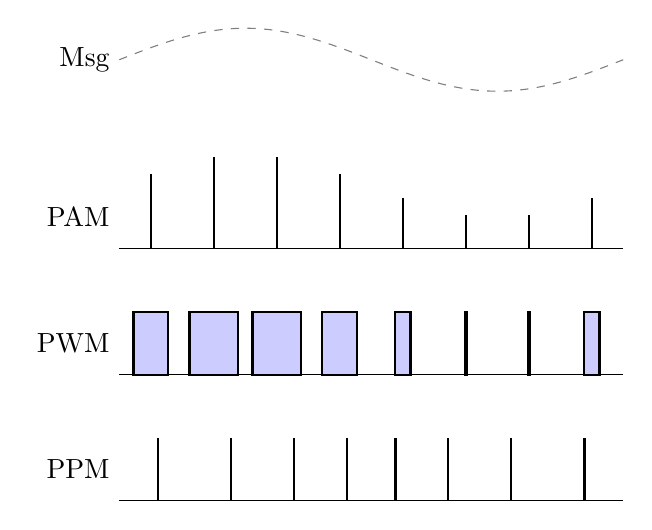
\begin{tikzpicture}[scale=0.8]
    % Message
    \draw[gray, dashed] plot[domain=0:8, samples=100] (\x, {1 + 0.5*sin(180*\x/4)});
    \node[left] at (0,1) {Msg};

    % PAM
    \begin{scope}[yshift=-2cm]
        \foreach \x in {0.5, 1.5, ..., 7.5} {
            \draw[thick] (\x,0) -- (\x, {1 + 0.5*sin(180*\x/4)});
        }
        \draw (0,0) -- (8,0);
        \node[left] at (0,0.5) {PAM};
    \end{scope}

    % PWM
    \begin{scope}[yshift=-4cm]
        \foreach \x in {0.5, 1.5, ..., 7.5} {
            \pgfmathsetmacro{\w}{0.2 + 0.2*sin(180*\x/4)}
            \draw[thick, fill=blue!20] (\x-\w, 0) rectangle (\x+\w, 1);
        }
        \draw (0,0) -- (8,0);
        \node[left] at (0,0.5) {PWM};
    \end{scope}

    % PPM
    \begin{scope}[yshift=-6cm]
        \foreach \x in {0.5, 1.5, ..., 7.5} {
             \pgfmathsetmacro{\s}{0.3*sin(180*\x/4)}
            \draw[thick] (\x+\s, 0) -- (\x+\s, 1);
        }
        \draw (0,0) -- (8,0);
        \node[left] at (0,0.5) {PPM};
    \end{scope}
\end{tikzpicture}
\captionof{figure}{Pulse Modulation Techniques}
\end{center}
\end{solutionbox}

\begin{mnemonicbox}
"AAA-PPW" - Amplitude, Position, Width are modulated in PAM, PPM, PWM
\end{mnemonicbox}

\questionmarks{3(a) OR}{3}{Define Nyquist rate and explain.}

\begin{solutionbox}
\textbf{Answer}:
Nyquist rate is the minimum sampling frequency required for accurate signal reconstruction.

\begin{center}
\captionof{table}{Nyquist Rate}
\begin{tabulary}{\linewidth}{|L|L|}
\hline
\textbf{Aspect} & \textbf{Description} \\
\hline
\textbf{Definition} & Minimum sampling frequency needed to avoid aliasing ($f_s = 2f_{max}$) \\
\hline
\textbf{Implications} & Sampling below Nyquist rate causes irreversible distortion \\
\hline
\textbf{Formula} & $f_s \ge 2f_{max}$ where $f_{max}$ is highest frequency in signal \\
\hline
\textbf{Application} & CD audio: 44.1 kHz sampling for 20 kHz audio \\
\hline
\end{tabulary}
\end{center}
\end{solutionbox}

\begin{mnemonicbox}
"TANS" - Twice As Needed for Sampling
\end{mnemonicbox}

\questionmarks{3(b) OR}{4}{Explain quantization process.}

\begin{solutionbox}
\textbf{Answer}:
Quantization assigns discrete amplitude levels to sampled values in analog-to-digital conversion.

\begin{center}
\captionof{table}{Quantization Process}
\begin{tabulary}{\linewidth}{|L|L|}
\hline
\textbf{Step} & \textbf{Description} \\
\hline
\textbf{Sampling} & Discrete-time samples taken from continuous signal \\
\hline
\textbf{Level Assignment} & Each sample assigned to nearest quantization level \\
\hline
\textbf{Quantization Error} & Difference between actual and quantized value \\
\hline
\textbf{Quantization Noise} & Statistical effect of errors in signal \\
\hline
\textbf{Resolution} & Determined by number of bits ($2^n$ levels for n bits) \\
\hline
\end{tabulary}
\end{center}

\begin{center}
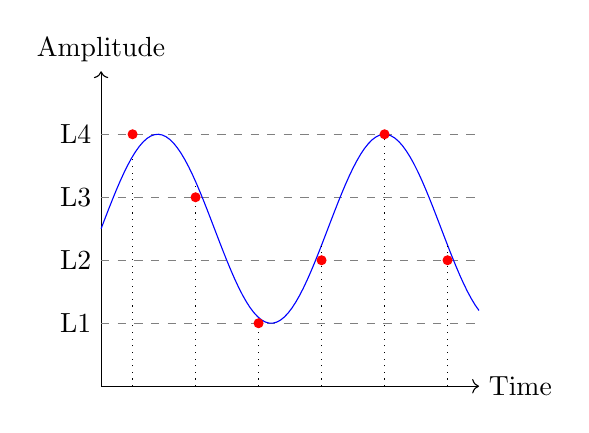
\begin{tikzpicture}[scale=0.8]
    \draw[->] (0,0) -- (6,0) node[right] {Time};
    \draw[->] (0,0) -- (0,5) node[above] {Amplitude};
    
    % Levels
    \foreach \y in {1,2,3,4} {
        \draw[dashed, gray] (0,\y) -- (6,\y);
        \node[left] at (0,\y) {L\y};
    }
    
    % Signal
    \draw[blue] plot[domain=0:6, samples=100] (\x, {2.5 + 1.5*sin(100*\x)});
    
    % Samples
    \foreach \x in {0.5, 1.5, ..., 5.5} {
        \draw[dotted] (\x,0) -- (\x, {2.5 + 1.5*sin(100*\x)});
        \filldraw[red] (\x, {round(2.5 + 1.5*sin(100*\x))}) circle (2pt);
    }
\end{tikzpicture}
\captionof{figure}{Quantization Process}
\end{center}
\end{solutionbox}

\begin{mnemonicbox}
"SLERN" - Sample, Level assign, Error occurs, Resolution determines Noise
\end{mnemonicbox}

\questionmarks{3(c) OR}{7}{Explain Ideal, Natural and Flat top sampling.}

\begin{solutionbox}
\textbf{Answer}:
These are different practical implementations of sampling process.

\begin{center}
\captionof{table}{Sampling Types Comparison}
\begin{tabulary}{\linewidth}{|L|L|L|L|}
\hline
\textbf{Type} & \textbf{Description} & \textbf{Characteristics} & \textbf{Mathematical Representation} \\
\hline
\textbf{Ideal} & Instantaneous samples at zero width & Theoretical concept, not physically realizable & $s(t) = m(t) \times \sum\delta(t-nT_s)$ \\
\hline
\textbf{Natural} & Samples modulate pulse train & Practical implementation using analog switch & $s(t) = m(t) \times p(t)$ \\
\hline
\textbf{Flat-top} & Holds sample value until next sample & Easiest to implement, sample-and-hold circuit & $s(t) = \sum m(nT_s)[u(t-nT_s)-u(t-(n+1)T_s)]$ \\
\hline
\end{tabulary}
\end{center}

\begin{center}
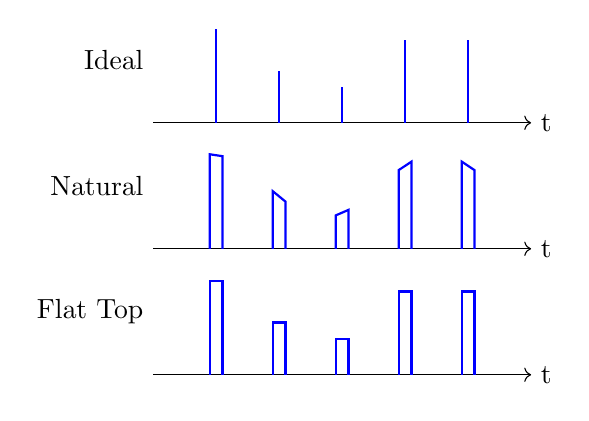
\begin{tikzpicture}[scale=0.8]
    % Ideal
    \begin{scope}[yshift=4cm]
        \draw[->] (0,0) -- (6,0) node[right] {t};
        \foreach \x in {1,2,3,4,5} \draw[thick, blue] (\x,0) -- (\x, {1+0.5*sin(100*\x)});
        \node[left] at (0,1) {Ideal};
    \end{scope}
    
    % Natural
    \begin{scope}[yshift=2cm]
        \draw[->] (0,0) -- (6,0) node[right] {t};
         \foreach \x in {1,2,3,4,5} {
            \draw[thick, blue] (\x-0.1,0) -- (\x-0.1, {1+0.5*sin(100*(\x-0.1))}) -- (\x+0.1, {1+0.5*sin(100*(\x+0.1))}) -- (\x+0.1, 0);
         }
         \node[left] at (0,1) {Natural};
    \end{scope}

    % Flat Top
    \begin{scope}[yshift=0cm]
        \draw[->] (0,0) -- (6,0) node[right] {t};
        \foreach \x in {1,2,3,4,5} {
            \draw[thick, blue] (\x-0.1,0) -- (\x-0.1, {1+0.5*sin(100*\x)}) -- (\x+0.1, {1+0.5*sin(100*\x)}) -- (\x+0.1, 0);
        }
        \node[left] at (0,1) {Flat Top};
    \end{scope}
\end{tikzpicture}
\captionof{figure}{Sampling Types}
\end{center}
\end{solutionbox}

\begin{mnemonicbox}
"INF" - Ideal is theoretical, Natural is practical, Flat-top holds values
\end{mnemonicbox}

\questionmarks{4(a)}{3}{List the advantages and disadvantages of PCM.}

\begin{solutionbox}
\textbf{Answer}:

\begin{center}
\captionof{table}{PCM Advantages and Disadvantages}
\begin{tabulary}{\linewidth}{|L|L|}
\hline
\textbf{Advantages} & \textbf{Disadvantages} \\
\hline
\textbf{High noise immunity} & Requires higher bandwidth \\
\hline
\textbf{Better signal quality} & Complex circuitry \\
\hline
\textbf{Compatible with digital systems} & Quantization noise \\
\hline
\textbf{Secure communication possible} & Higher power consumption \\
\hline
\textbf{Can be regenerated without degradation} & Synchronization required \\
\hline
\end{tabulary}
\end{center}
\end{solutionbox}

\begin{mnemonicbox}
"NICHE" vs "BCQPS" - Noise immunity, Integration, Complex circuitry, Higher bandwidth, Error correction vs Bandwidth, Cost, Quantization, Power, Synchronization
\end{mnemonicbox}

\questionmarks{4(b)}{4}{Draw and Explain Block Diagram of Delta Modulation.}

\begin{solutionbox}
\textbf{Answer}:
Delta modulation transmits only changes in signal level using 1-bit quantization.

\begin{center}
\begin{tikzpicture}[auto, >=latex, thick]
    \node (input) {Input};
    \node [draw, circle, right of=input] (sum) {$\Sigma$};
    \node [gtu block, right of=sum, node distance=2.5cm] (quant) {1-bit Quantizer};
    \node [right of=quant, node distance=2cm] (out) {Output};
    
    \node [gtu block, below of=quant] (int) {Integrator};
    \node [gtu block, below of=sum] (delay) {Delay};

    \draw [gtu arrow] (input) -- (sum);
    \draw [gtu arrow] (sum) -- (quant);
    \draw [gtu arrow] (quant) -- (out);
    \draw [gtu arrow] (quant) |- (int);
    \draw [gtu arrow] (int) -- (delay);
    \draw [gtu arrow] (delay) -- node {$-\,$} (sum);
\end{tikzpicture}
\captionof{figure}{Delta Modulation Block Diagram}
\end{center}

\begin{center}
\captionof{table}{Delta Modulation Components}
\begin{tabulary}{\linewidth}{|L|L|}
\hline
\textbf{Block} & \textbf{Function} \\
\hline
\textbf{Comparator} & Compares input with predicted value \\
\hline
\textbf{1-bit Quantizer} & Outputs 1 if difference positive, 0 if negative \\
\hline
\textbf{Integrator} & Accumulates step values to track input \\
\hline
\textbf{Delay} & Provides previous output for comparison \\
\hline
\end{tabulary}
\end{center}
\end{solutionbox}

\begin{mnemonicbox}
"CQID" - Compare, Quantize with 1-bit, Integrate, Delay
\end{mnemonicbox}

\questionmarks{4(c)}{7}{Compare PCM, DM and DPCM.}

\begin{solutionbox}
\textbf{Answer}:

\begin{center}
\captionof{table}{Comparison of Digital Modulation Techniques}
\begin{tabulary}{\linewidth}{|L|L|L|L|}
\hline
\textbf{Parameter} & \textbf{PCM} & \textbf{DM} & \textbf{DPCM} \\
\hline
\textbf{Bits per sample} & 8-16 bits & 1 bit & 4-6 bits \\
\hline
\textbf{Bandwidth} & Highest & Lowest & Medium \\
\hline
\textbf{Signal-to-Noise Ratio} & Highest & Lowest & Medium \\
\hline
\textbf{Circuit Complexity} & High & Simple & Medium \\
\hline
\textbf{Sampling Rate} & Nyquist & Multiple of Nyquist & Nyquist \\
\hline
\textbf{Error Types} & Quantization error & Slope overload, granular noise & Prediction error \\
\hline
\textbf{Applications} & CD audio, digital telephony & Low-quality voice & Speech, video coding \\
\hline
\end{tabulary}
\end{center}
\end{solutionbox}

\begin{mnemonicbox}
"PCM-DM-DPCM: More Bits Better Quality, More Complexity Needed"
\end{mnemonicbox}

\questionmarks{4(a) OR}{3}{Explain DPCM.}

\begin{solutionbox}
\textbf{Answer}:
Differential Pulse Code Modulation encodes difference between actual and predicted sample.

\begin{center}
\captionof{table}{DPCM Characteristics}
\begin{tabulary}{\linewidth}{|L|L|}
\hline
\textbf{Aspect} & \textbf{Description} \\
\hline
\textbf{Basic Principle} & Encodes difference between actual and predicted value \\
\hline
\textbf{Predictor} & Uses previous samples to predict current value \\
\hline
\textbf{Advantage} & Requires fewer bits than PCM (exploits correlation) \\
\hline
\textbf{Bit Rate Reduction} & Typically 25-50\% compared to PCM \\
\hline
\textbf{Applications} & Speech coding, image compression \\
\hline
\end{tabulary}
\end{center}
\end{solutionbox}

\begin{mnemonicbox}
"DPCM: Difference Predicted, Correlation Matters"
\end{mnemonicbox}

\questionmarks{4(b) OR}{4}{List the advantages and disadvantages of Delta Modulation.}

\begin{solutionbox}
\textbf{Answer}:

\begin{center}
\captionof{table}{Delta Modulation - Pros and Cons}
\begin{tabulary}{\linewidth}{|L|L|}
\hline
\textbf{Advantages} & \textbf{Disadvantages} \\
\hline
\textbf{Simple implementation} & Slope overload distortion \\
\hline
\textbf{Low bit rate} & Granular noise at low amplitudes \\
\hline
\textbf{Single bit transmission} & Limited dynamic range \\
\hline
\textbf{Robust against channel errors} & Higher sampling rate required \\
\hline
\textbf{Low complexity hardware} & Lower SNR than PCM \\
\hline
\end{tabulary}
\end{center}
\end{solutionbox}

\begin{mnemonicbox}
"SLSRL" vs "SGLSH" - Simple, Low bit-rate, Single bit, Robust, Low cost vs Slope overload, Granular noise, Limited range, Sampling high, SNR low
\end{mnemonicbox}

\questionmarks{4(c) OR}{7}{Explain Block diagram of basic PCM-TDM system.}

\begin{solutionbox}
\textbf{Answer}:
PCM-TDM combines multiple digitized signals into a single high-speed channel.

\begin{center}
\begin{tikzpicture}[auto, >=latex, thick, scale=0.9, transform shape]
    \node (in1) {In 1};
    \node [gtu block, right of=in1] (enc1) {PCM 1};
    \node [below of=in1, node distance=1.5cm] (in2) {In 2};
    \node [gtu block, right of=in2] (enc2) {PCM 2};
    
    \node [gtu block, right of=enc1, yshift=-0.75cm, minimum height=2.5cm] (mux) {TDM \\ MUX};
    \node [right of=mux, node distance=2.5cm] (ch) {Channel};
    \node [gtu block, right of=ch, node distance=2.5cm, minimum height=2.5cm] (demux) {TDM \\ DEMUX};
    
    \node [gtu block, right of=demux, yshift=0.75cm] (dec1) {Dec 1};
    \node [right of=dec1] (out1) {Out 1};
    \node [gtu block, right of=demux, yshift=-0.75cm] (dec2) {Dec 2};
    \node [right of=dec2] (out2) {Out 2};
    
    \draw [gtu arrow] (in1) -- (enc1);
    \draw [gtu arrow] (in2) -- (enc2);
    \draw [gtu arrow] (enc1) -- (mux.160);
    \draw [gtu arrow] (enc2) -- (mux.200);
    \draw [gtu arrow] (mux) -- (ch) -- (demux);
    \draw [gtu arrow] (demux.20) -- (dec1);
    \draw [gtu arrow] (demux.340) -- (dec2);
    \draw [gtu arrow] (dec1) -- (out1);
    \draw [gtu arrow] (dec2) -- (out2);
\end{tikzpicture}
\captionof{figure}{PCM-TDM System Block Diagram}
\end{center}

\begin{center}
\captionof{table}{PCM-TDM System Components}
\begin{tabulary}{\linewidth}{|L|L|}
\hline
\textbf{Block} & \textbf{Function} \\
\hline
\textbf{PCM Encoder} & Converts analog signal to digital (sampling, quantization, coding) \\
\hline
\textbf{TDM Multiplexer} & Combines multiple PCM streams into single high-speed stream \\
\hline
\textbf{Transmission Channel} & Medium for signal transmission \\
\hline
\textbf{TDM Demultiplexer} & Separates time-multiplexed stream back into individual channels \\
\hline
\textbf{PCM Decoder} & Converts digital back to analog (decoding, filtering) \\
\hline
\textbf{Synchronization} & Clock and frame sync signals ensure proper demultiplexing \\
\hline
\textbf{Frame Structure} & Contains samples from all channels plus sync bits \\
\hline
\end{tabulary}
\end{center}
\end{solutionbox}

\begin{mnemonicbox}
"PETDSF" - PCM Encodes, TDM combines, Digital transmits, Separation occurs, Frames synchronize
\end{mnemonicbox}

\questionmarks{5(a)}{3}{Explain Adaptive Delta Modulation.}

\begin{solutionbox}
\textbf{Answer}:
Adaptive Delta Modulation adjusts step size based on signal characteristics.

\begin{center}
\captionof{table}{Adaptive Delta Modulation}
\begin{tabulary}{\linewidth}{|L|L|}
\hline
\textbf{Feature} & \textbf{Description} \\
\hline
\textbf{Basic Principle} & Varies step size according to signal slope \\
\hline
\textbf{Step Size Control} & Increases when same bit pattern repeats (signal changing rapidly) \\
\hline
\textbf{Advantages} & Reduced slope overload and granular noise \\
\hline
\textbf{Implementation} & Uses shift register to detect bit patterns \\
\hline
\textbf{Performance} & Better SNR than standard DM \\
\hline
\end{tabulary}
\end{center}

\begin{center}
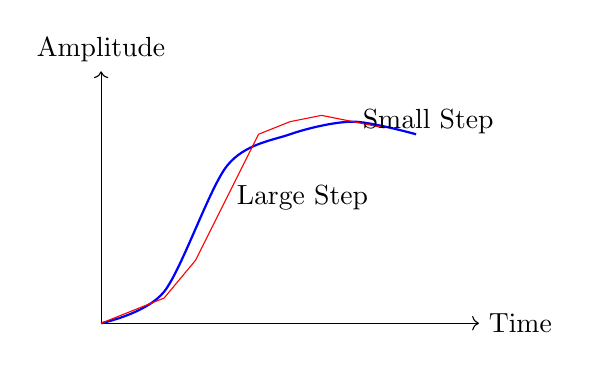
\begin{tikzpicture}[scale=0.8]
    \draw[->] (0,0) -- (6,0) node[right] {Time};
    \draw[->] (0,0) -- (0,4) node[above] {Amplitude};
    
    \draw[blue, thick] plot [smooth] coordinates {(0,0) (1,0.5) (2,2.5) (3,3) (4,3.2) (5,3)};
    
    \draw[red] (0,0) -- (0.5, 0.2) -- (1, 0.4) -- (1.5, 1.0) -- (2, 2.0) -- (2.5, 3.0) -- (3, 3.2) -- (3.5, 3.3) -- (4, 3.2) -- (4.5, 3.1);
    
    \node[right] at (2, 2.0) {Large Step};
    \node[right] at (4, 3.2) {Small Step};
\end{tikzpicture}
\captionof{figure}{Step Size Adaptation}
\end{center}
\end{solutionbox}

\begin{mnemonicbox}
"ASSG" - Adaptive Step Size Gives better performance
\end{mnemonicbox}

\questionmarks{5(b)}{4}{Define the terms: 1. Radiation Pattern 2. Antenna Gain.}

\begin{solutionbox}
\textbf{Answer}:

\begin{center}
\captionof{table}{Antenna Terms}
\begin{tabulary}{\linewidth}{|L|L|L|}
\hline
\textbf{Term} & \textbf{Definition} & \textbf{Characteristics} \\
\hline
\textbf{Radiation Pattern} & Graphical representation of radiation properties of antenna in space & Shows directional dependencies of radiated power \\
\hline
\textbf{Antenna Gain} & Measure of antenna's ability to direct or concentrate radio energy in a particular direction & Expressed in dB, compared to isotropic radiator (dBi) \\
\hline
\end{tabulary}
\end{center}

\begin{center}
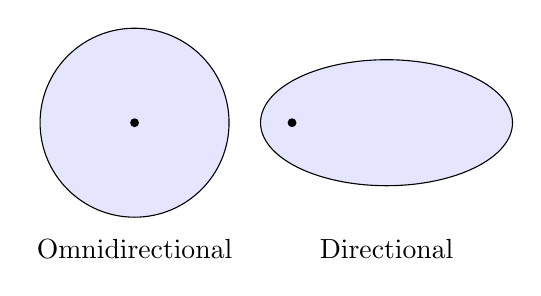
\begin{tikzpicture}[scale=0.8]
    % Omni
    \begin{scope}
        \draw[fill=blue!10] (0,0) circle (1.5);
        \fill (0,0) circle (2pt);
        \node[below] at (0,-1.7) {Omnidirectional};
    \end{scope}
    
    % Directional
    \begin{scope}[xshift=4cm]
        \draw[fill=blue!10] (0,0) ellipse (2 and 1);
        \fill (-1.5,0) circle (2pt);
        \node[below] at (0,-1.7) {Directional};
    \end{scope}
\end{tikzpicture}
\captionof{figure}{Radiation Pattern Types}
\end{center}
\end{solutionbox}

\begin{mnemonicbox}
"RPGD" - Radiation Pattern shows Gain Direction
\end{mnemonicbox}

\questionmarks{5(c)}{7}{Explain Base station and mobile station antennas.}

\begin{solutionbox}
\textbf{Answer}:
Different antenna designs serve different purposes in wireless communication systems.

\begin{center}
\captionof{table}{Comparison of Base Station and Mobile Station Antennas}
\begin{tabulary}{\linewidth}{|L|L|L|}
\hline
\textbf{Parameter} & \textbf{Base Station Antenna} & \textbf{Mobile Station Antenna} \\
\hline
\textbf{Height} & 15-50 meters & Less than 2 meters \\
\hline
\textbf{Gain} & Higher (10-20 dBi) & Lower (0-3 dBi) \\
\hline
\textbf{Pattern} & Sectoral (120$^\circ$ sectors) & Omnidirectional \\
\hline
\textbf{Size} & Larger arrays & Compact, integrated \\
\hline
\textbf{Types} & Panel, Yagi, Collinear & Monopole, PIFA, chip \\
\hline
\textbf{Polarization} & Vertical, cross-polarized & Typically vertical \\
\hline
\textbf{Beamforming} & Often used & Rarely used in basic devices \\
\hline
\textbf{Diversity} & Space/polarization diversity & Rarely implemented \\
\hline
\end{tabulary}
\end{center}
\end{solutionbox}

\begin{mnemonicbox}
"BHPSTBD" - Base stations Have Power, Size, Tower mounting, Beamforming, Diversity
\end{mnemonicbox}

\questionmarks{5(a) OR}{3}{Write frequency range for HF, VHF and UHF.}

\begin{solutionbox}
\textbf{Answer}:

\begin{center}
\captionof{table}{Frequency Bands}
\begin{tabulary}{\linewidth}{|L|L|L|L|}
\hline
\textbf{Band} & \textbf{Frequency Range} & \textbf{Wavelength} & \textbf{Notable Applications} \\
\hline
\textbf{HF} & 3-30 MHz & 100-10 m & Shortwave radio, amateur radio, aviation \\
\hline
\textbf{VHF} & 30-300 MHz & 10-1 m & FM radio, TV channels 2-13, air traffic \\
\hline
\textbf{UHF} & 300-3000 MHz & 1-0.1 m & TV channels 14-83, mobile phones, Wi-Fi \\
\hline
\end{tabulary}
\end{center}
\end{solutionbox}

\begin{mnemonicbox}
"3-30-300-3000" - Each band starts at 3 times a power of 10 MHz
\end{mnemonicbox}

\questionmarks{5(b) OR}{4}{Define the terms: 1. Antenna Directivity 2. Polarization.}

\begin{solutionbox}
\textbf{Answer}:

\begin{center}
\captionof{table}{Antenna Properties}
\begin{tabulary}{\linewidth}{|L|L|L|}
\hline
\textbf{Term} & \textbf{Definition} & \textbf{Characteristics} \\
\hline
\textbf{Directivity} & Ratio of radiation intensity in a given direction to average radiation intensity & Measured in dBi, indicates focus of antenna \\
\hline
\textbf{Polarization} & Orientation of electric field vector of radiated wave & Linear (vertical/horizontal), circular, elliptical \\
\hline
\end{tabulary}
\end{center}

\begin{center}
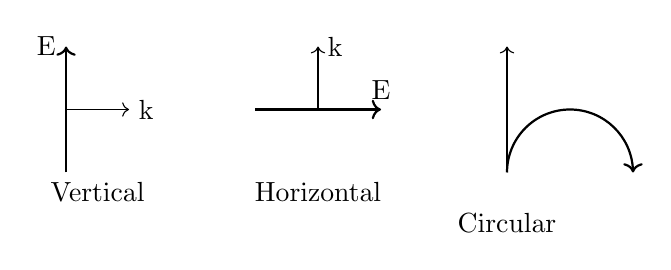
\begin{tikzpicture}[scale=0.8]
    % Vertical
    \draw[thick, ->] (0,0) -- (0,2) node[left] {E};
    \draw[->] (0,1) -- (1,1) node[right] {k};
    \node[below] at (0.5,0) {Vertical};
    
    % Horizontal
    \begin{scope}[xshift=3cm]
        \draw[thick, ->] (0,1) -- (2,1) node[above] {E};
        \draw[->] (1,1) -- (1,2) node[right] {k};
        \node[below] at (1,0) {Horizontal};
    \end{scope}
    
    % Circular
    \begin{scope}[xshift=7cm]
        \draw[thick, ->] (0,0) arc (180:0:1);
        \draw[->] (0,0) -- (0,2);
        \node[below] at (0,-0.5) {Circular};
    \end{scope}
\end{tikzpicture}
\captionof{figure}{Antenna Directivity and Polarization}
\end{center}
\end{solutionbox}

\begin{mnemonicbox}
"DIVE POLE" - DIrectivity shows Vector Excellence, POLarization shows Electric field
\end{mnemonicbox}

\questionmarks{5(c) OR}{7}{Explain Ground wave and Space wave propagation in detail.}

\begin{solutionbox}
\textbf{Answer}:
These are two primary modes of radio wave propagation in the lower atmosphere.

\begin{center}
\captionof{table}{Wave Propagation Comparison}
\begin{tabulary}{\linewidth}{|L|L|L|}
\hline
\textbf{Parameter} & \textbf{Ground Wave} & \textbf{Space Wave} \\
\hline
\textbf{Frequency Range} & Below 2 MHz & Above 30 MHz \\
\hline
\textbf{Distance Coverage} & 100-300 km & Limited to line-of-sight + diffraction \\
\hline
\textbf{Path} & Follows earth's curvature & Direct and ground-reflected paths \\
\hline
\textbf{Mechanism} & Diffraction around earth's surface & Line-of-sight propagation with reflection \\
\hline
\textbf{Attenuation} & Higher (increases with frequency) & Lower at VHF/UHF ranges \\
\hline
\textbf{Polarization} & Vertical polarization preferred & Both vertical and horizontal usable \\
\hline
\textbf{Applications} & AM broadcasting, navigation beacons & TV, FM radio, microwave links \\
\hline
\textbf{Factors Affecting} & Ground conductivity, terrain & Antenna height, terrain, obstacles \\
\hline
\end{tabulary}
\end{center}

\begin{center}
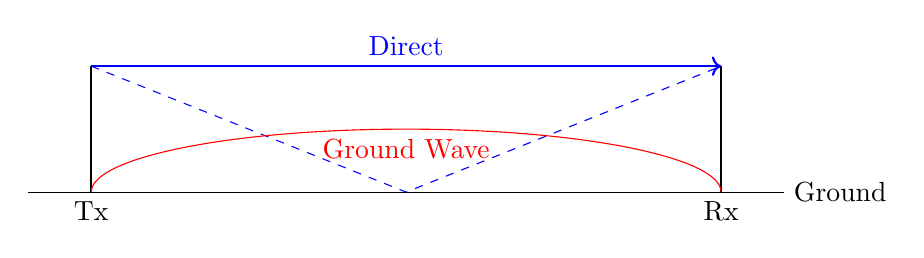
\begin{tikzpicture}[scale=0.8]
    \draw (-6,0) -- (6,0) node[right] {Ground};
    
    % TX
    \draw[thick] (-5,0) -- (-5,2);
    \node[below] at (-5,0) {Tx};
    
    % RX
    \draw[thick] (5,0) -- (5,2);
    \node[below] at (5,0) {Rx};
    
    % Space Wave Direct
    \draw[blue, thick, ->] (-5,2) -- (5,2) node[midway, above] {Direct};
    
    % Space Wave Reflected
    \draw[blue, dashed] (-5,2) -- (0,0) -- (5,2);
    
    % Ground Wave
    \draw[red] (-5,0) arc (180:0:5 and 1);
    \node[red, below] at (0,1) {Ground Wave};
\end{tikzpicture}
\captionof{figure}{Ground Wave vs Space Wave Propagation}
\end{center}

\textbf{Ground Wave Propagation:}
\begin{itemize}
    \item Travels along the surface of the earth.
    \item Signal strength decreases with distance.
    \item Better propagation over sea than land.
    \item Affected by ground conductivity and dielectric constant.
    \item Used for AM broadcasting, Maritime communication.
\end{itemize}

\textbf{Space Wave Propagation:}
\begin{itemize}
    \item Involves Direct Wave and Ground-Reflected Wave.
    \item Range extended by atmospheric refraction.
    \item Range formula: $d = \sqrt{2Rh}$ where R is earth radius, h is antenna height.
    \item Affected by diffraction over obstacles.
    \item Used for Line-of-sight communication like TV, FM, Microwave links.
\end{itemize}
\end{solutionbox}

\begin{mnemonicbox}
"GAFFS" - Ground Adheres to earth, Follows surface, Frequencies low, Short wavelengths
\end{mnemonicbox}

\end{document}



